\begin{tikzpicture}[thick]
	
	\pgfmathsetlengthmacro{\sep}{2.5em}
	
	\pgfmathsetlengthmacro{\labelsep}{0.5em}
	\tikzset{widelabel/.style={ font=\footnotesize
	                      , align=center
	                      , inner sep=0
	                      }}
	\tikzset{label/.style={ widelabel
	                      , text width=3cm
	                      }}
	
	
	% Callout from #1 to callout box #2 from corner #3 to #4 and corner
	% #5 to #6
	\tikzset{glow/.style={line width=1.0mm,white}}
	\newcommand{\callout}[6]{
		\draw [glow] (#2.north west) rectangle (#2.south east);
		\draw [glow] (#1.#3) -- (#2.#4);
		\draw [glow] (#1.#5) -- (#2.#6);
		
		\draw        (#2.north west) rectangle (#2.south east);
		\draw        (#1.#3) -- (#2.#4);
		\draw        (#1.#5) -- (#2.#6);
	}
	
	\newcommand{\hcallout}[2]{
		\callout{#1}{#2}{north east}{north west}{south east}{south west}
	}
	\newcommand{\vcallout}[2]{
		\callout{#1}{#2}{south east}{north east}{south west}{north west}
	}
	
	% A mess of neurons
	\node (neurons) [inner sep=0]
	      {\input{|"python2 figures/random-network.py 10 25 25 5 0.2 100 3 0.2 1.0"}}
	      ;
	
	% A SpiNNaker die
	\node (die) [inner sep=0]
	      [right=\sep of neurons]
	      {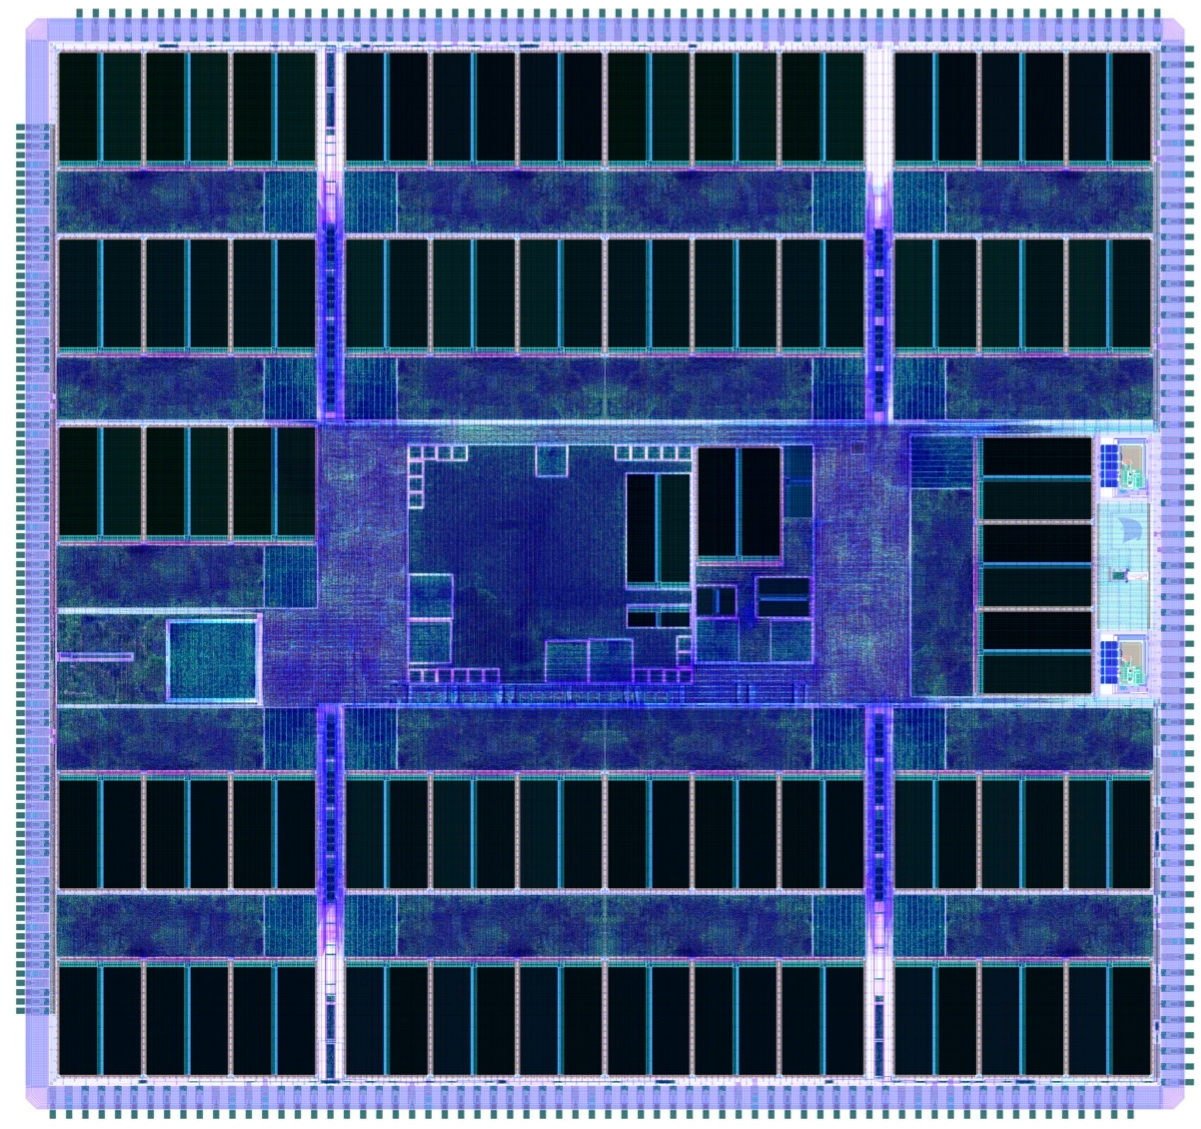
\includegraphics[height=3cm]{figures/spinnakerDie}};
	\node (core) at ([shift={(5.0mm,1.5mm)}]die.west)
	      [ inner sep=0
	      , minimum width =7mm
	      , minimum height=5mm
	      ]
	      {};
	\hcallout{neurons}{core}
	
	% A SpiNNaker board
	\node (board) [inner sep=0]
	      [right=\sep of die]
	      {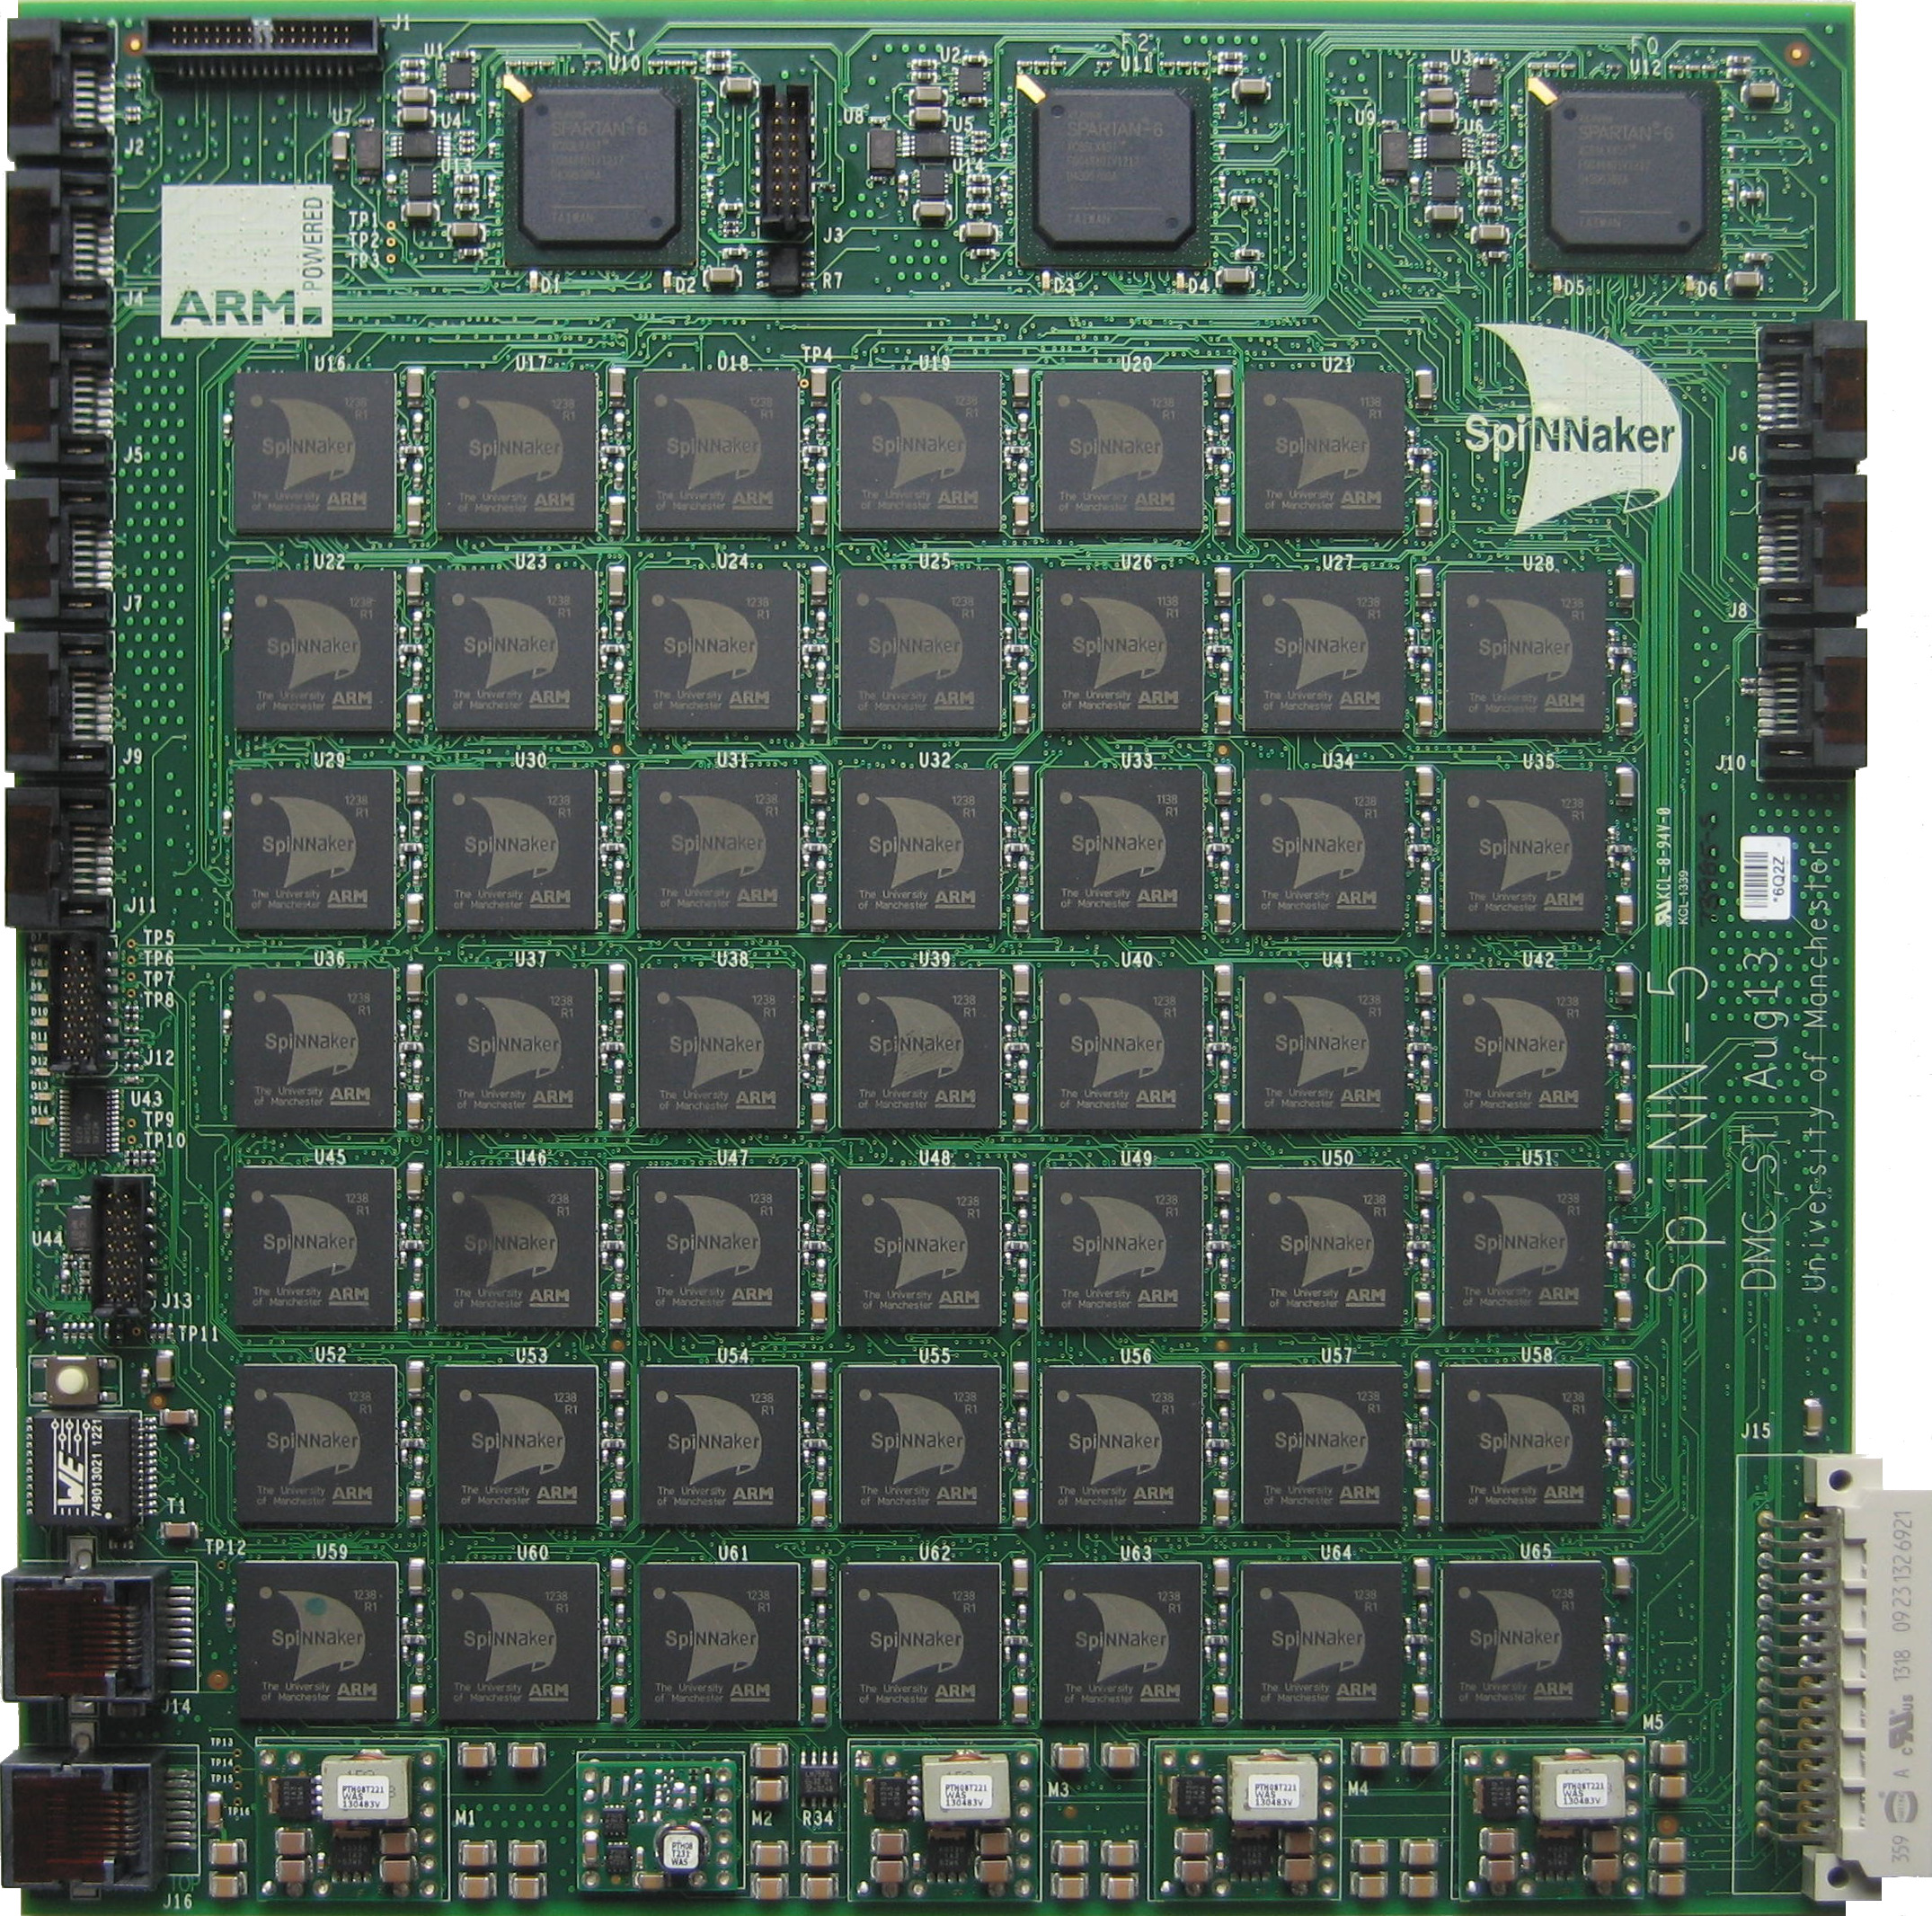
\includegraphics[height=3cm]{figures/spinnakerBoard}};
	\node (chip) at ([shift={(5.0mm,1.6mm)}]board.west)
	      [ inner sep=0
	      , minimum width =3mm
	      , minimum height=3mm
	      ]
	      {};
	\hcallout{die}{chip}
	
	% A rack of boards
	\node (rack) [inner sep=0]
	      [right=\sep of board]
	      {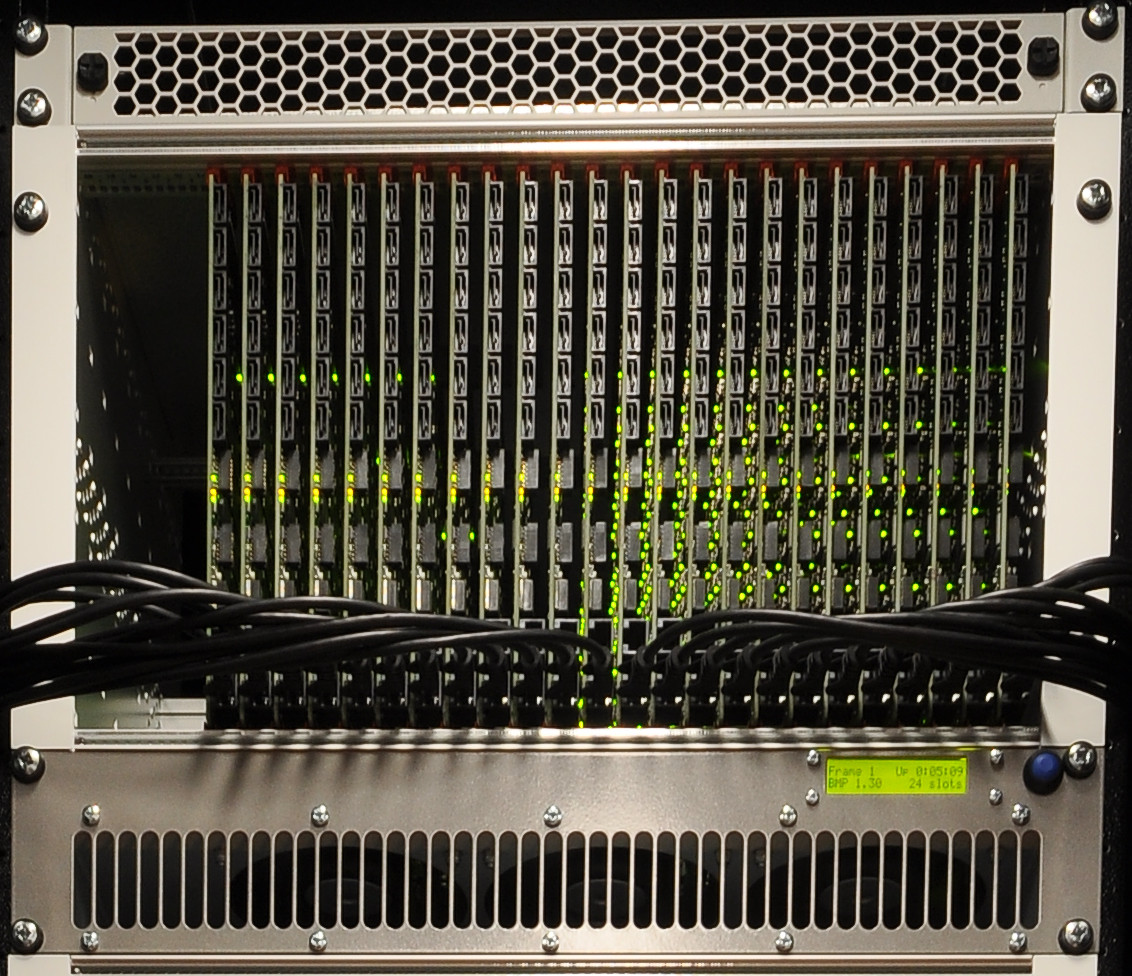
\includegraphics[height=3cm]{figures/spinnakerRack}};
	\node (fitted board) at ([shift={(7mm,2mm)}]rack.west)
	      [ inner sep=0
	      , minimum width =1mm
	      , minimum height=16mm
	      ]
	      {};
	\hcallout{board}{fitted board}
	
	% A ten cabinet machine
	\coordinate (top row) at ($(neurons.south west)!0.5!(rack.south east)$);
	\node (cabinet) [inner sep=0]
	      [below=\sep of top row]
	      {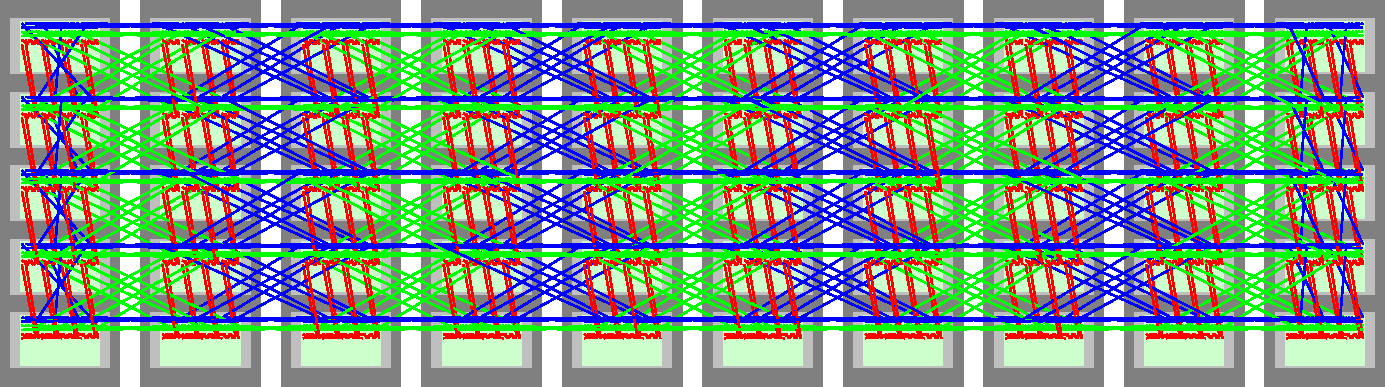
\includegraphics[width=\textwidth]{figures/spinnaker106}};
	\node (fitted rack) at ([shift={(-23.2mm,-5.5mm)}]cabinet.north east)
	      [ inner sep=0
	      , minimum width =11.5mm
	      , minimum height=6.5mm
	      ]
	      {};
	\vcallout{rack}{fitted rack}
	
	% Labels
	\node [above=\labelsep of neurons, label] {1,000 neurons \\ per core.};
	\node [above=\labelsep of die, label] {18 cores \\ per chip.};
	\node [above=\labelsep of board, label] {48 chips \\ per board.};
	\node [above=\labelsep of rack, label] {24 boards \\ per rack.};
	\node [below=\labelsep of cabinet, widelabel] {5 racks per cabinet, 10
	cabinets.};
	
\end{tikzpicture}

